\section{PI Force Controller}
In this section the results for the PI Force Controller are presented. First a summary of results is given for each scenario presented in Section \ref{sec:PI}. Then three different comparisons that were studied are presented one of PI vs PID performance, support vs non-support simulation, 1s vs 3s Simulation. 

\subsubsection{Figure Layout Explanation}
Before diving into the results it is important to have a clear understanding of the image layout. The oval shape represented in the figures symbolizes the patient's body and the lines provide a basic representation of the arm (see Figure \ref{fig:armsimplification}). 

The green dot resembles the start of the movement and the red dot the end. The large blue dot indicates the desired position, while the series of smaller blue dots trace the arm's trajectory. 

The PI controller was successfully implemented across 64 points (see Figure \ref{fig:create_grid}).

\subsection{Scenario 1: From equilibrium position to target without Neural Excitation}
Scenario 1 was simulated during 3 seconds with a time step of 0.001s, Kp = 2000 and Ki = 100 (See Table \ref{tab:PI}).
The PI model successfully controlled the force for the 64 positions reaching. The table below presents performance results from Scenario 1.

\begin{table}[h]
    \centering
    \caption{Results for PI Controller Without Neural Excitation from Equilibrium Position to Target Position}
    \scriptsize
    \begin{tabularx}{\textwidth}{|l|X|X|}
        \hline
        \textbf{Parameter} & \textbf{Mean} & \textbf{Variance} \\        
        \hline

        Target Position Error (m) & [-0.0026 -0.0022 -0.0041] & [0.206 0.2916 0.3936]$*10^{-4}$ \\
        Steady State Time (s) & 0.4066 & 0.0093 \\
        Simulation Time (s) & 4.91 & 0.0093        \\
        \hline

    \end{tabularx}

    \label{tab:PINNE}
\end{table}

It can be seen that the mean target position error is very low and there is not a high variance for the 64 different positions. Moreover, the steady force values are achieved early during the simulation. Finally, it is interesting to highlight that the simulation running time has a 2s difference from the real-time simulation. 

The GIF \ref{gif:PICONTROLLER2} (best viewed in Adobe Acrobat) illustrated the OpenSIM movement under the PI controller without neural excitation from equilibrium position to target position. 


\begin{figure}[h!]
    \centering
    \animategraphics[autoplay,loop,width=0.75\textwidth]{12}{Pictures/Results/NoExct/frame_}{11}{45}
    \caption{PI Controller No Excitation from Equilibrium Position. Open in Adobe Acrobat to see gif movement.}
    \label{gif:PICONTROLLER2}

\end{figure}

\newpage
\subsection{Scenario 2: Holding initial position with different muscles Neural Excitation}
Scenario 2 was simulated during 0.5 seconds with a time step of 0.001s, Kp = 2000 and Ki = 100 (See Table \ref{tab:PI}).
The PI model successfully controlled the force for the 64 positions. The table below presents some results from Scenario 2 for the 9 muscle categories.
\begin{table}[h]
    \centering
    \tiny % Set font size
    \caption{Results for PI Controller With Neural Excitation to Hold Static Position for Each Muscle}
    \begin{tabularx}{\linewidth}{|l|X|X|X|X|X|X|}
        \hline
        & \multicolumn{2}{c|}{\textbf{Target Position Error (m)}} & \multicolumn{2}{c|}{\textbf{Steady State Time (s)}} & \multicolumn{2}{c|}{\textbf{Simulation Time (s)}} \\
        \cline{2-7}
        \textbf{Muscle Group} & \textbf{Mean} & \textbf{Variance} & \textbf{Mean} & \textbf{Variance} & \textbf{Mean} & \textbf{Variance} \\
        \hline
        Triceps & [0.005 0.006 0.027] & [0.244 0.08 0.054]$*10^{-3}$ &  0.100 & 0.027 & 2.80 & 0.070 \\
        \hline
        Serratus Anterior & [ 0.001 -0.001 0.004] & [0.146 0.339 0.054]$*10^{-4}$ &  0.201 & 0.005 & 2.86 & 0.126 \\
        \hline
        Biceps/ Brachialis & [0.001 -0.002 -0.012] & [0.219 0.191 0.04]$*10^{-3}$ &  0.143 & 0.027 & 2.89 & 0.048 \\
        \hline
        Supra/ Infraspinatus & [-0.027 -0.018 0.013] & [0.104 0.06 0.110]$*10^{-3}$ & 0.229 & 0.025  & 3.07 & 0.088 \\
        \hline
        Rhomboids & [0.000 0.000 0.002] & [0.132 0.342 0.065]$*10^{-4}$ &   0.219 & 0.003 & 2.97 & 0.028 \\
        \hline
        Lower Pectoralis & [0.023 -0.010 0.002] & [0.110 0.293 0.199]$*10^{-3}$ &  0.131 & 0.035 & 2.90 & 0.105 \\
        \hline
        Upper Pectoralis & [0.008 -0.007 0.006] & [0.258 0.242 0.291]$*10^{-4}$ &   0.216 & 0.029 & 2.87 & 0.070 \\
        \hline
        None & [0.000 0.000 0.002] & [0.137 0.314 0.053]$*10^{-4}$ &  0.207 & 0.004 & 2.72 & 0.033 \\
        \hline
    \end{tabularx}
    \label{table:PIResults}
\end{table}

\begin{figure}[h]
    \centering
    \animategraphics[autoplay,loop,width=0.75\textwidth]{12}{Pictures/Results/TricepsExct/frame_}{0}{34}
    \caption{PI Controller maintaining Static Position with Triceps Excitation. Open in Adobe Acrobat to see gif movement.}
    \label{gif:PICONTROLLER1}
\end{figure}

The GIF \ref{gif:PICONTROLLER1} (best viewed in Adobe Acrobat) illustrated the OpenSIM movement under the PI controller  maintaining the position during triceps stimulation.

The average target position error remains very low with a low variance still for the 64 different positions. In addition, the PI controller is able to find the force that will maintain a steady state in half of the simulation time. However, the real simulation time is more than high times higher than the simulated time. This could be because when a matrix singularity is found the system is reset with different initial arm length values. This could delay the process of simulation. 

\newpage
\subsection{PI vs PID Controller}

In the evaluation process for optimizing PI parameters, it was observed that integrating the derivative term (D) of the PID controller did not yield significant improvements in performance with respect to target position, simulation time or reaching a steady position time. The only difference is that the PID presents lower variance with respect to the target position but the difference is not very substantial. 

As a result, the simpler PI model was adopted. A comparison between PI and PID performances is provided in the accompanying image. For the PI model, the constants utilized were Kp = 2000 and Ki = 100 and for the PID model the Kd=300.

\begin{table}[h]
    \centering
    \tiny % Set font size
    \caption{Comparison between PI and PID Controller Results}
    \begin{tabularx}{\linewidth}{|l|X|X|X|X|X|X|}
        \hline
        & \multicolumn{2}{c|}{\textbf{Target Position Error (m)}} & \multicolumn{2}{c|}{\textbf{Steady State Time (s)}} & \multicolumn{2}{c|}{\textbf{Simulation Time (s)}} \\
        \cline{2-7}
        \textbf{Controller} & \textbf{Mean} & \textbf{Variance} & \textbf{Mean} & \textbf{Variance} & \textbf{Mean} & \textbf{Variance} \\
        \hline
        PID & [0.000 -0.001 0.002] & [0.01 0.027 0.05]$*10^{-4}$ &  0.230 & 0.004 & 2.73 & 0.064 \\
        \hline
        PI  & [0.000 0.000 0.002] & [0.137 0.314 0.053]$*10^{-4}$ &  0.207 & 0.004 & 2.72 & 0.033 \\
        \hline
    \end{tabularx}
\end{table}

\begin{figure}[h!]
    \centering

   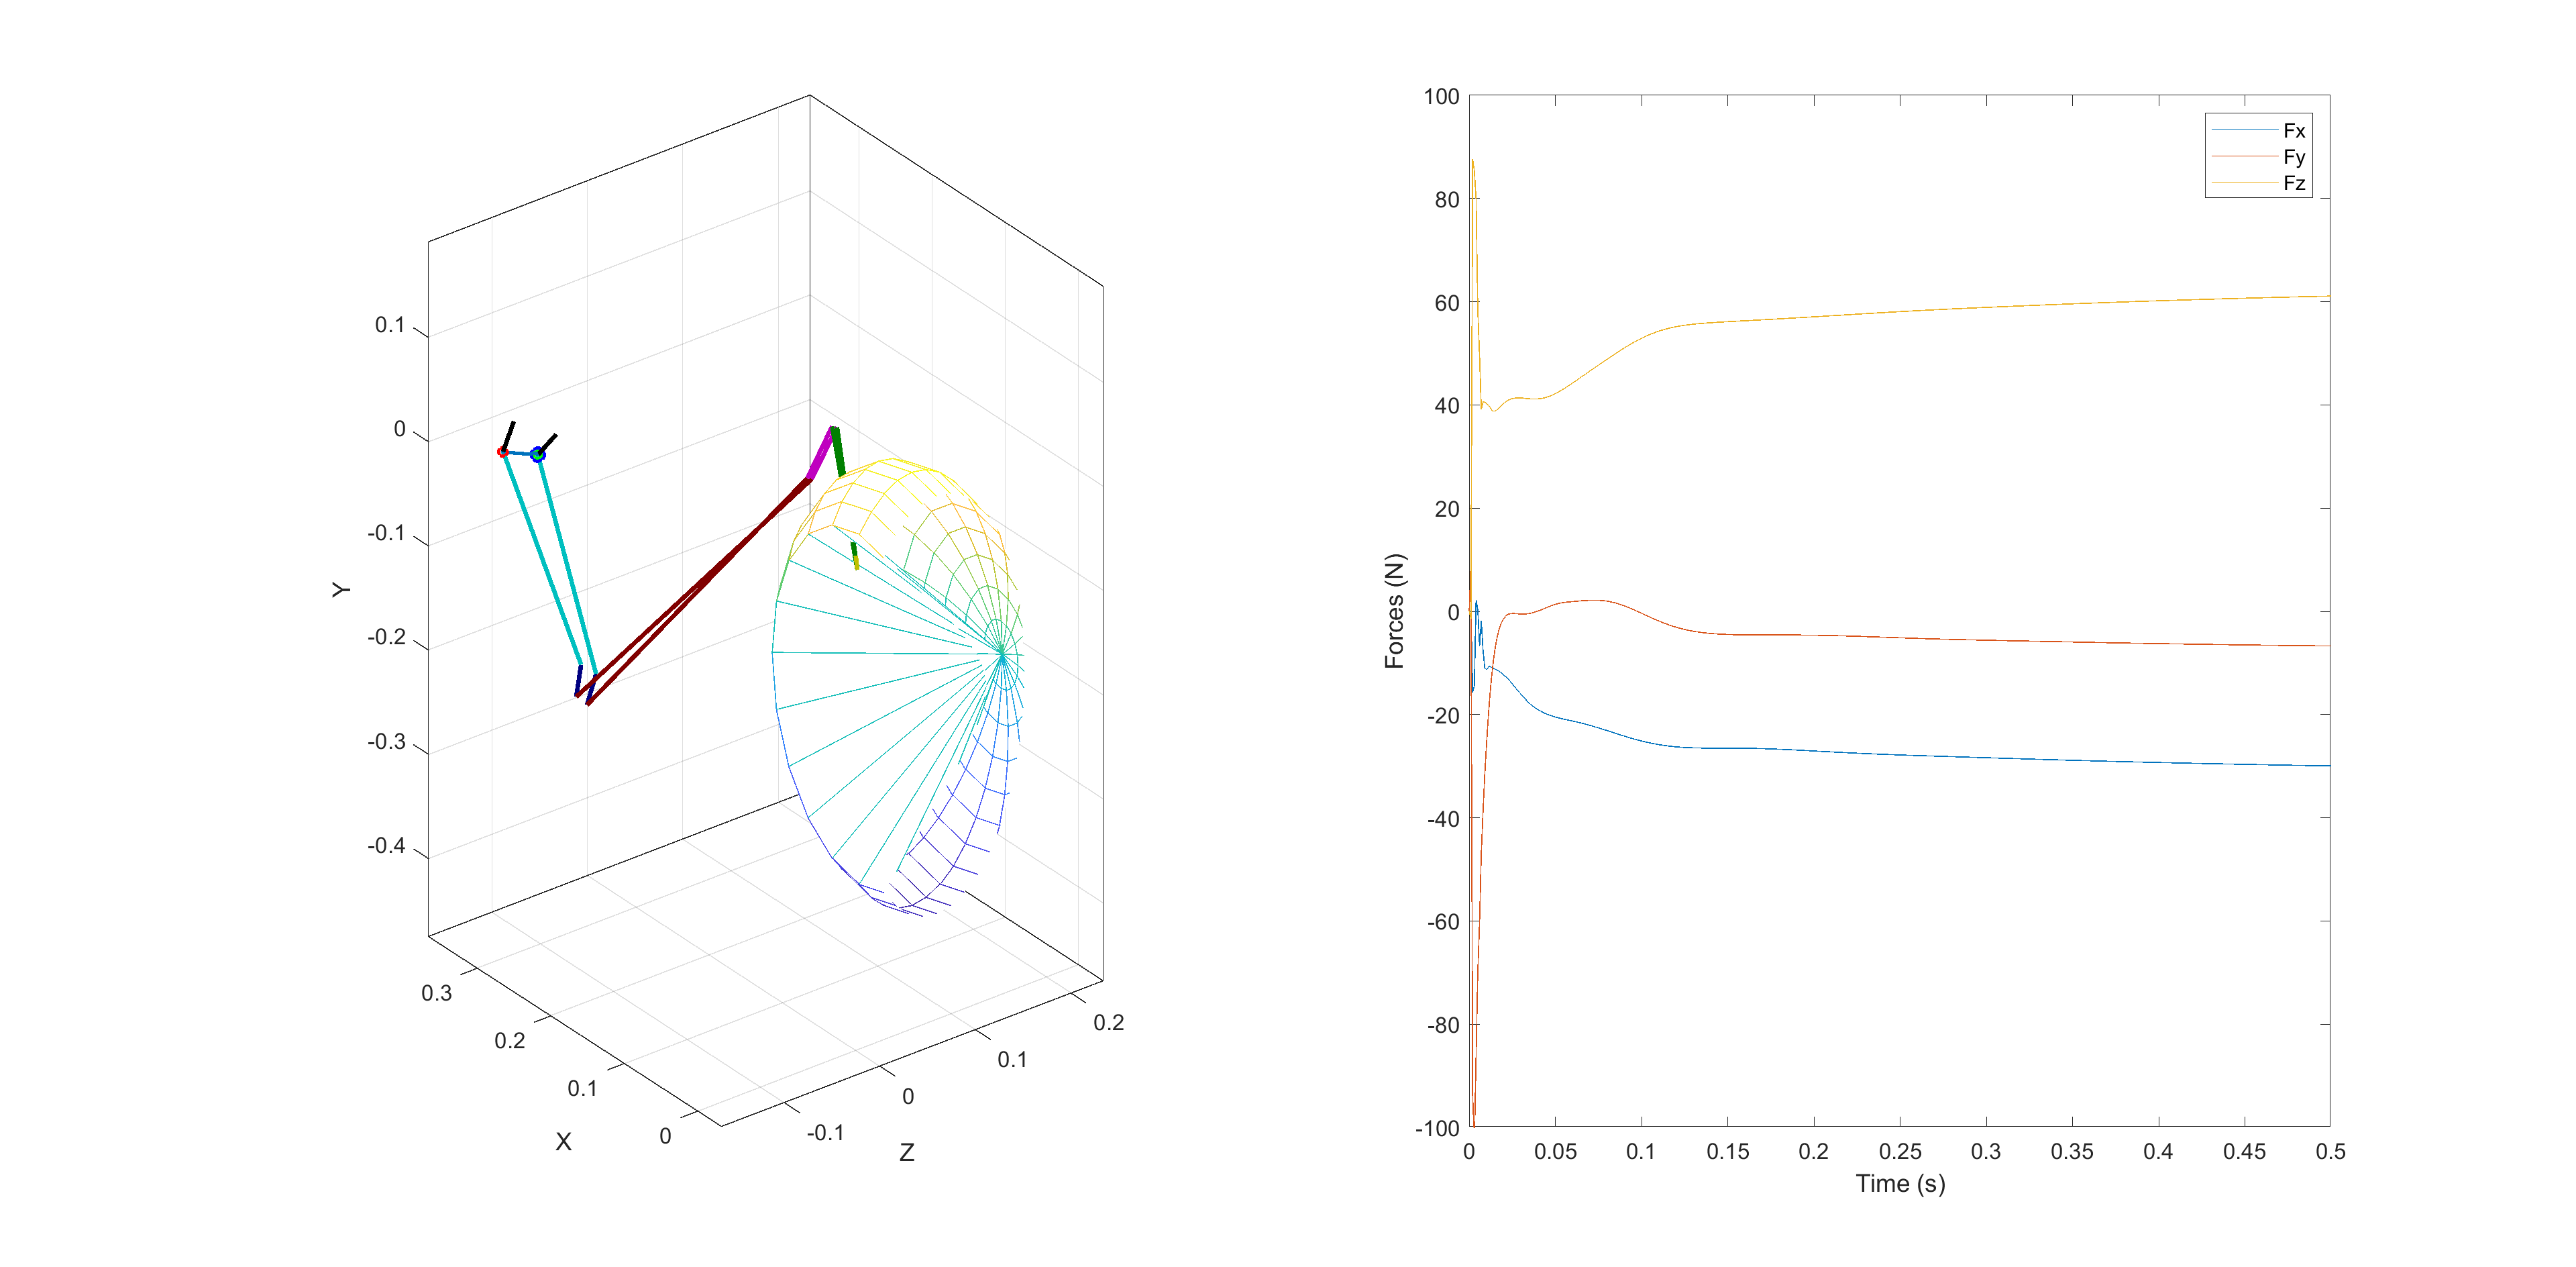
\includegraphics[width=0.8\linewidth]{Pictures/Results/PIDController_NeuralExcitation.png}
    \caption{PID Controller Holding Static Position with One Muscle Excitation.}
\end{figure}

\begin{figure}[h!]  
    \centering

    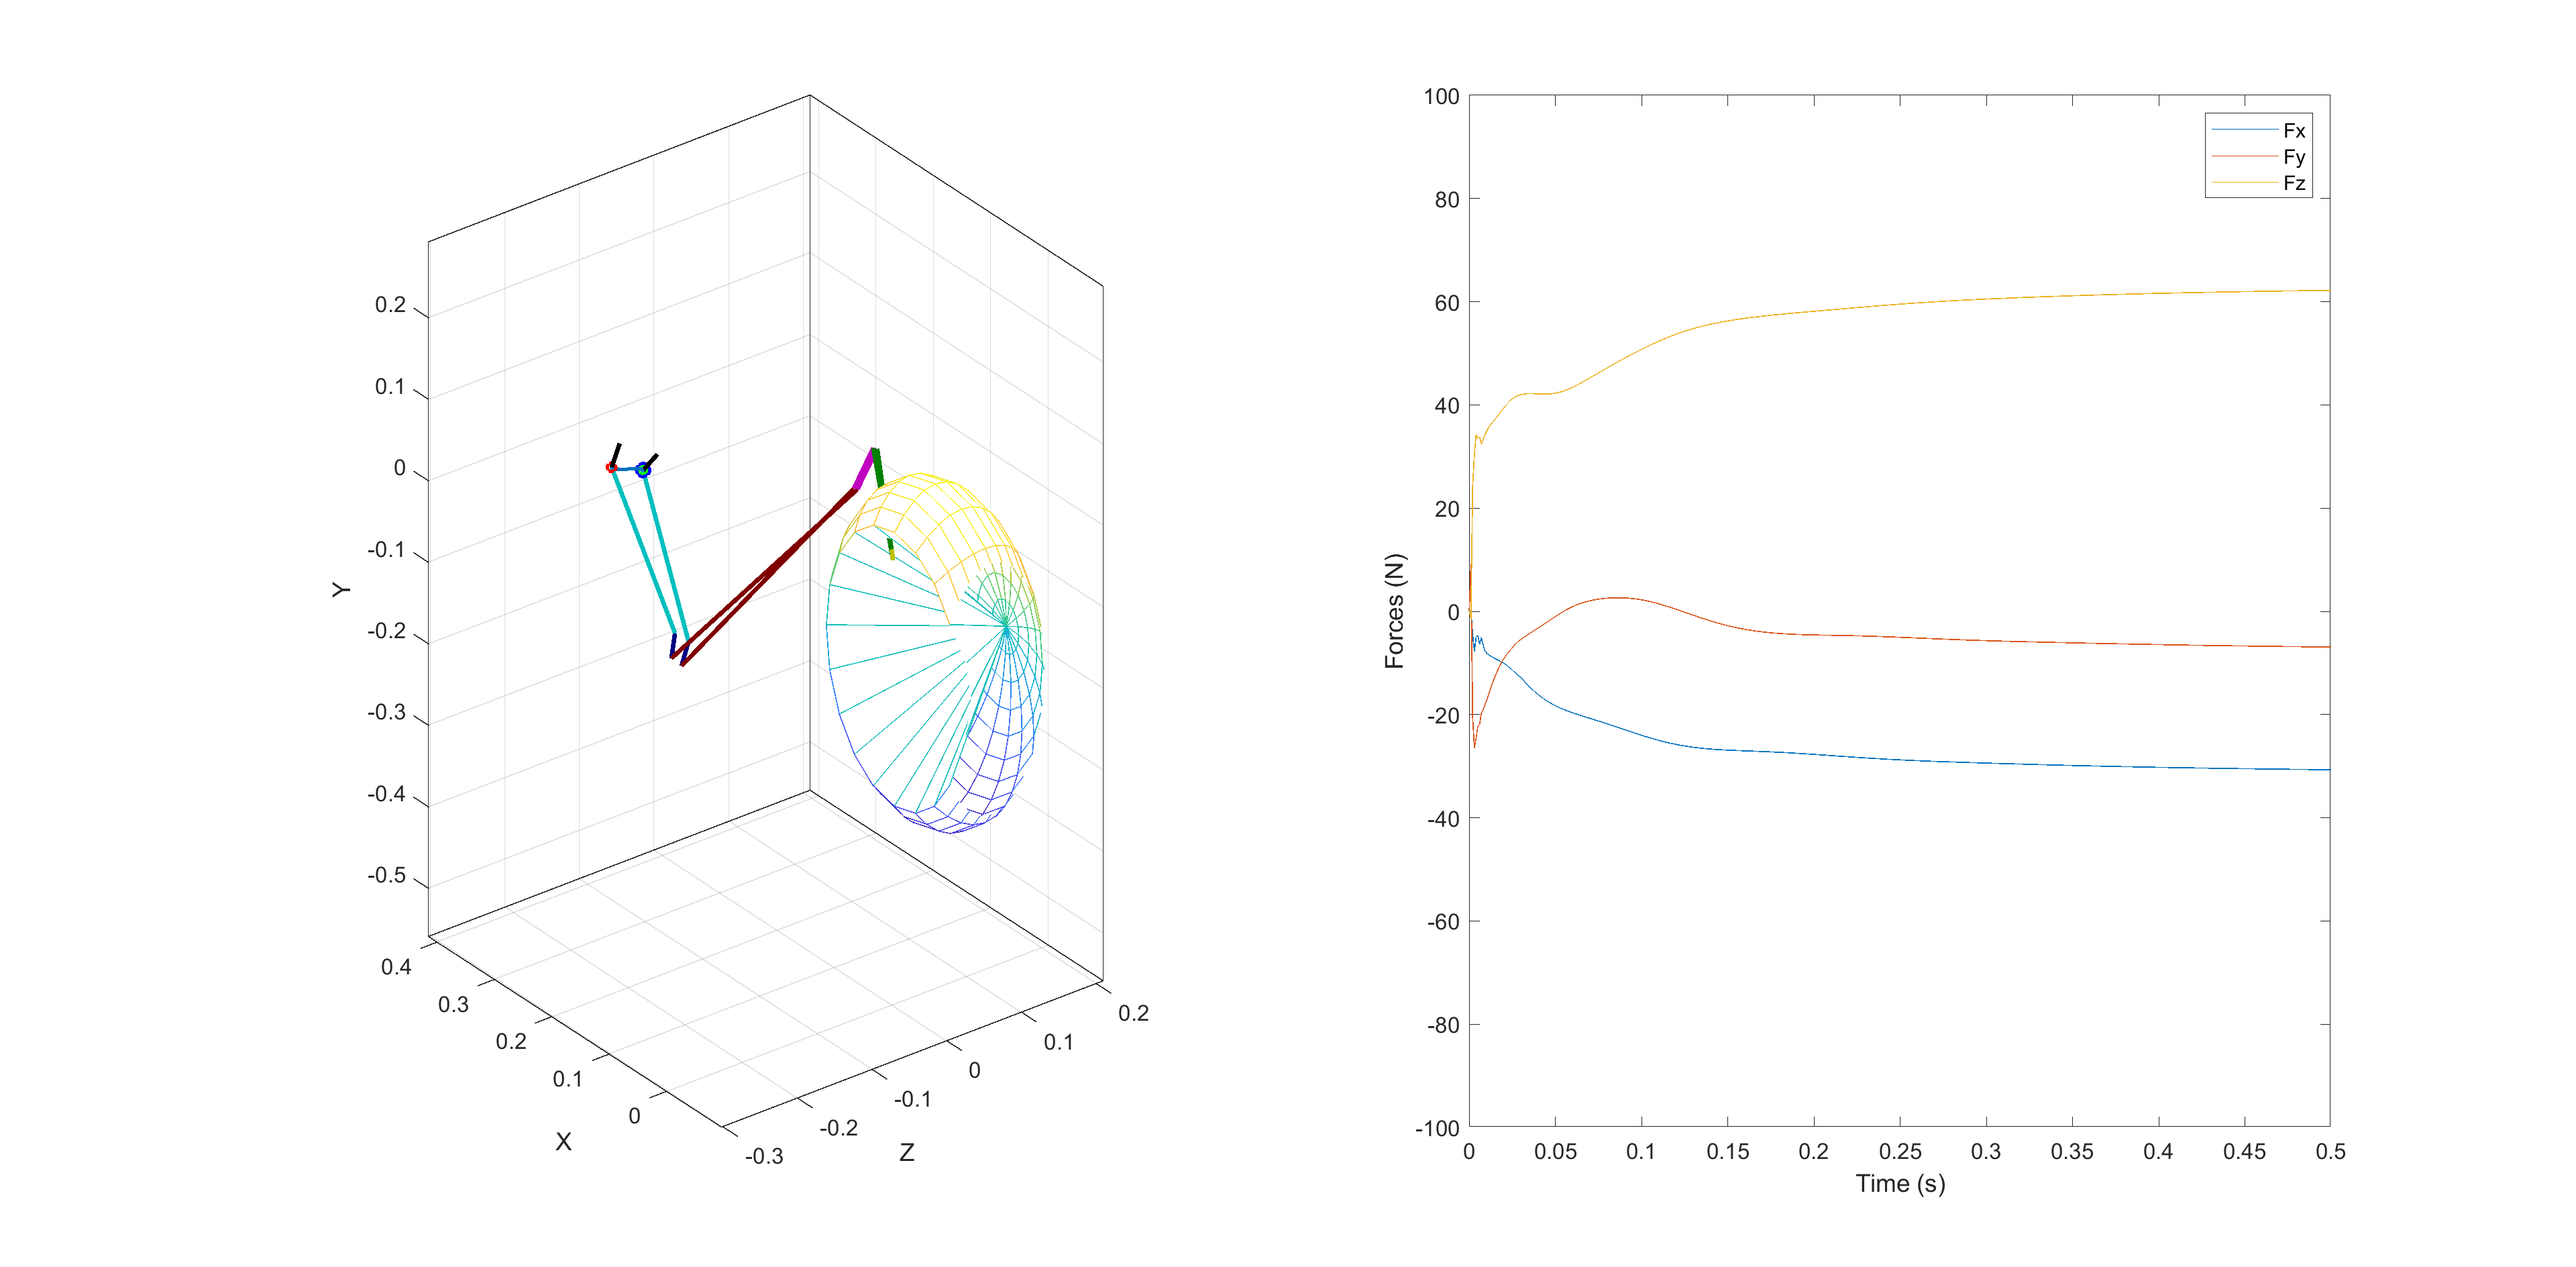
\includegraphics[width=0.8\linewidth]{Pictures/Results/PIController_NeuralExcitation.png}
    \caption{PI Controller Holding Static Position with One Muscle Excitation.}
\end{figure}



\newpage
\subsection{1s vs 3s Duration for Simulations Without Neural Excitation}

Initially, simulations were conducted over a 3-second duration. However, upon iterative testing, it was discerned that a duration of 1 second was sufficient. This conclusion is supported by the information seen on Table \ref{table:PIResults} The introduction of arm support reinforced this observation, as a marked reduction in oscillations was noted, leading to faster arm stabilization. A comparative analysis between scenarios with and without arm support is explored in the subsequent section.

\begin{figure}[h!]
    \centering

   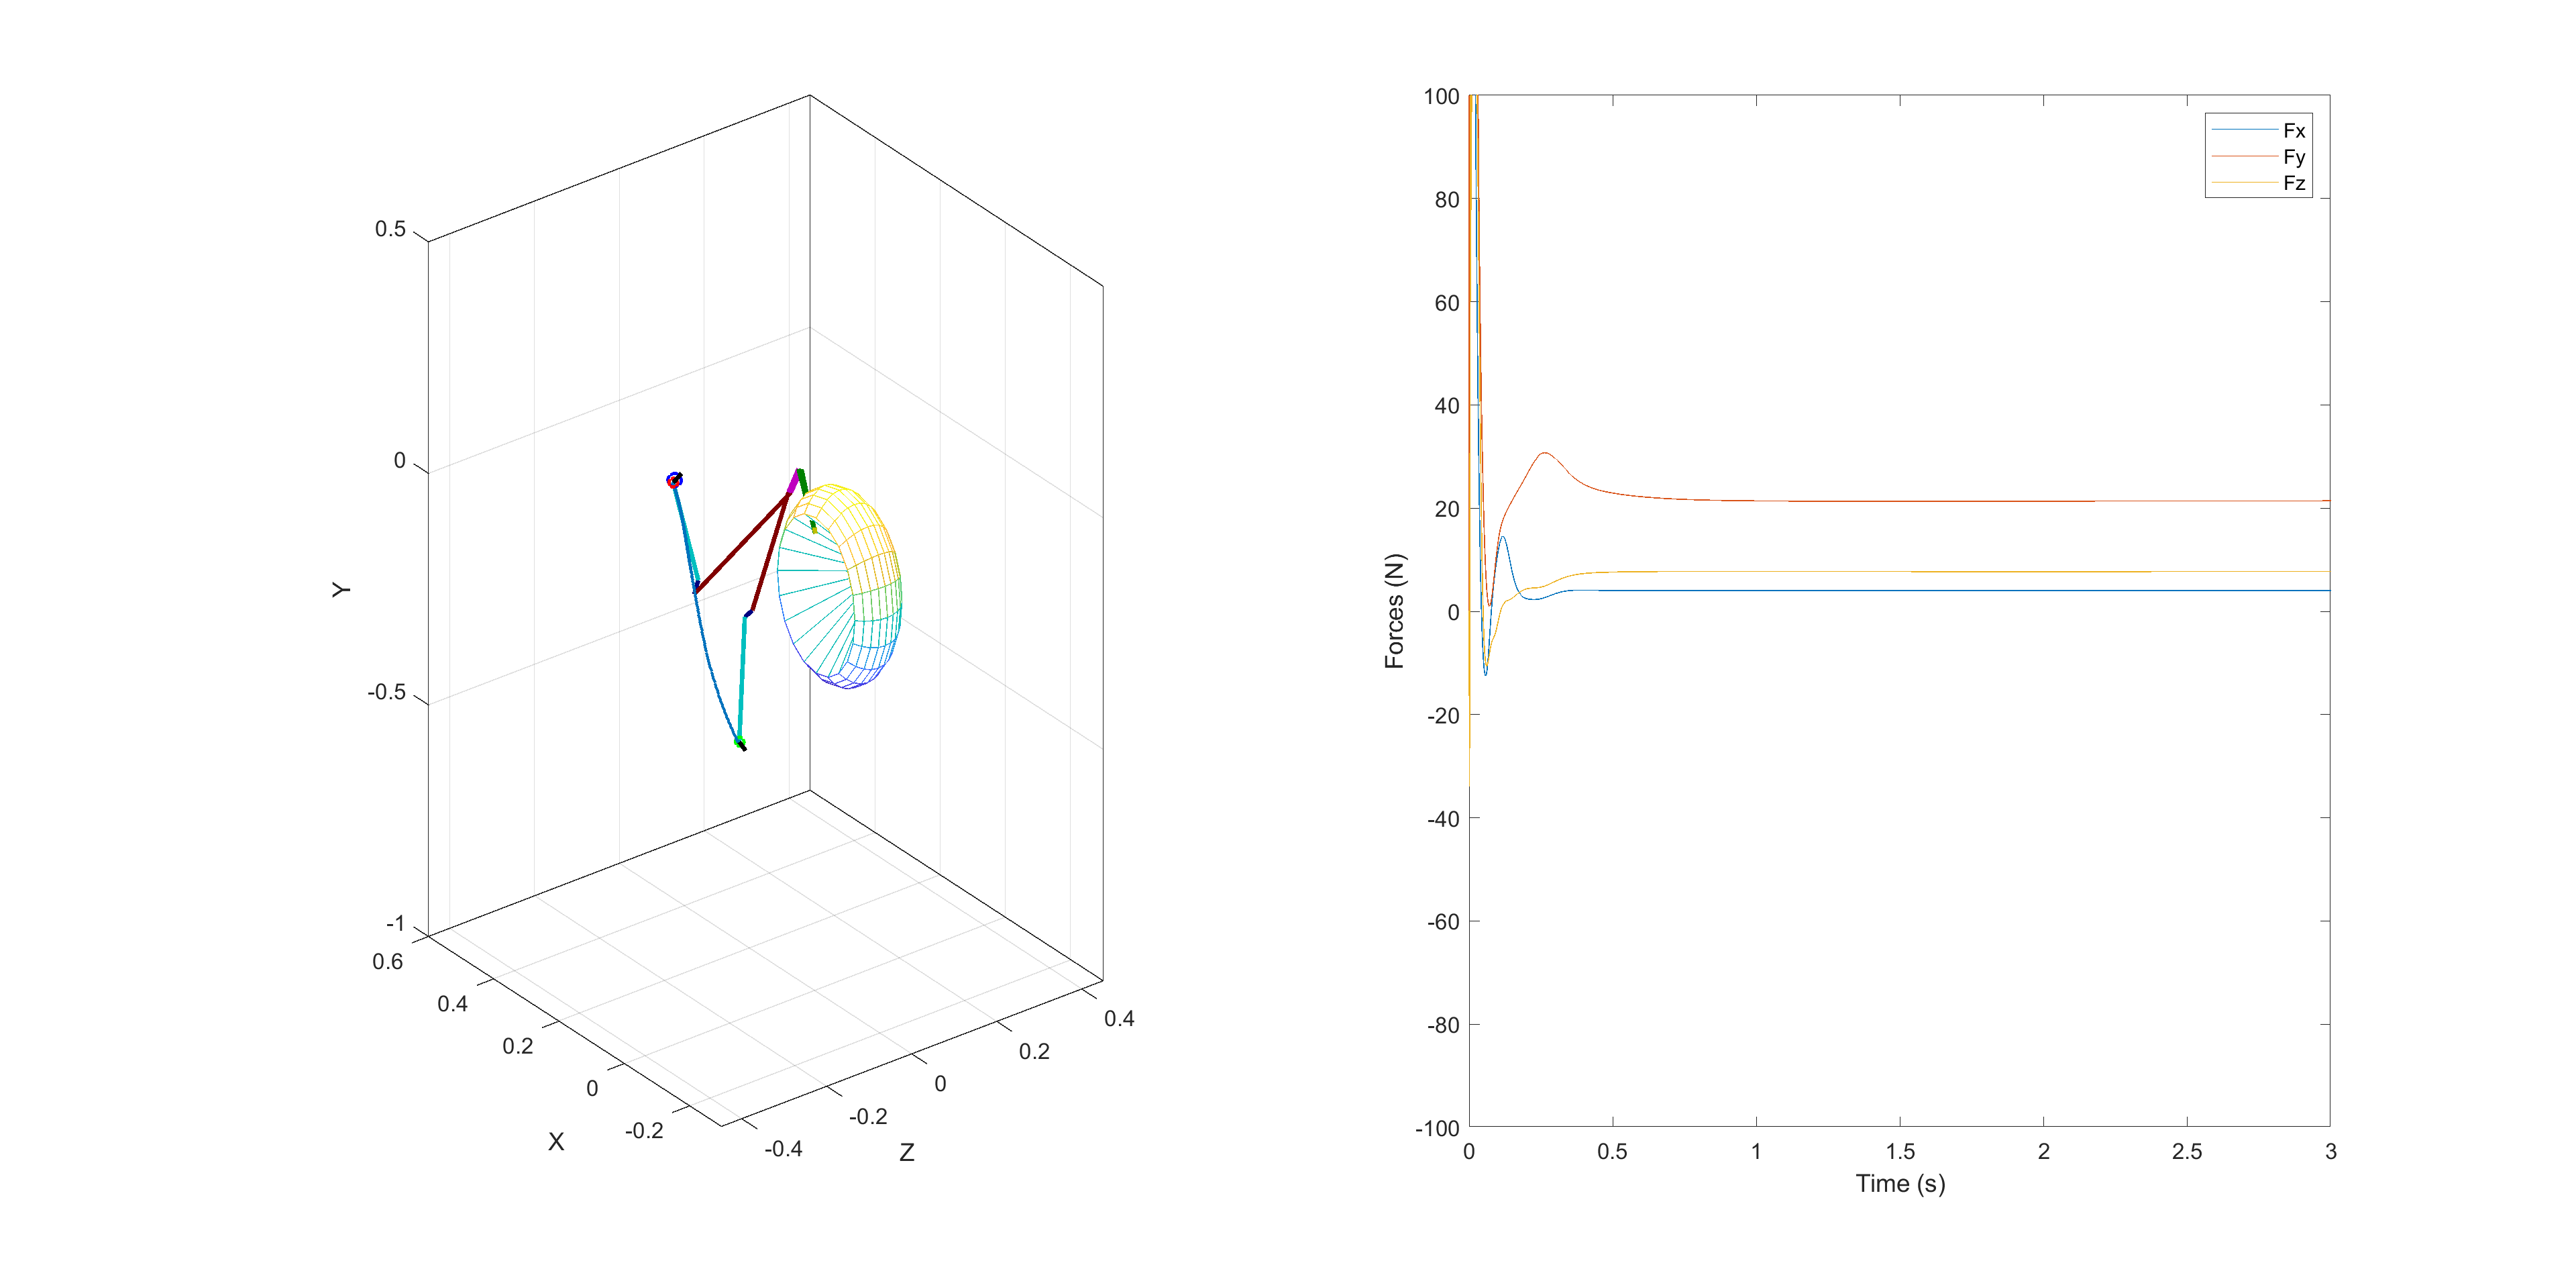
\includegraphics[width=0.7\linewidth]{Pictures/Results/3s_NoNeuralExcitation.png}
    \caption{PI Controller 3 seconds Simulation.}
\end{figure}

\begin{figure}[h!]    
    \centering
    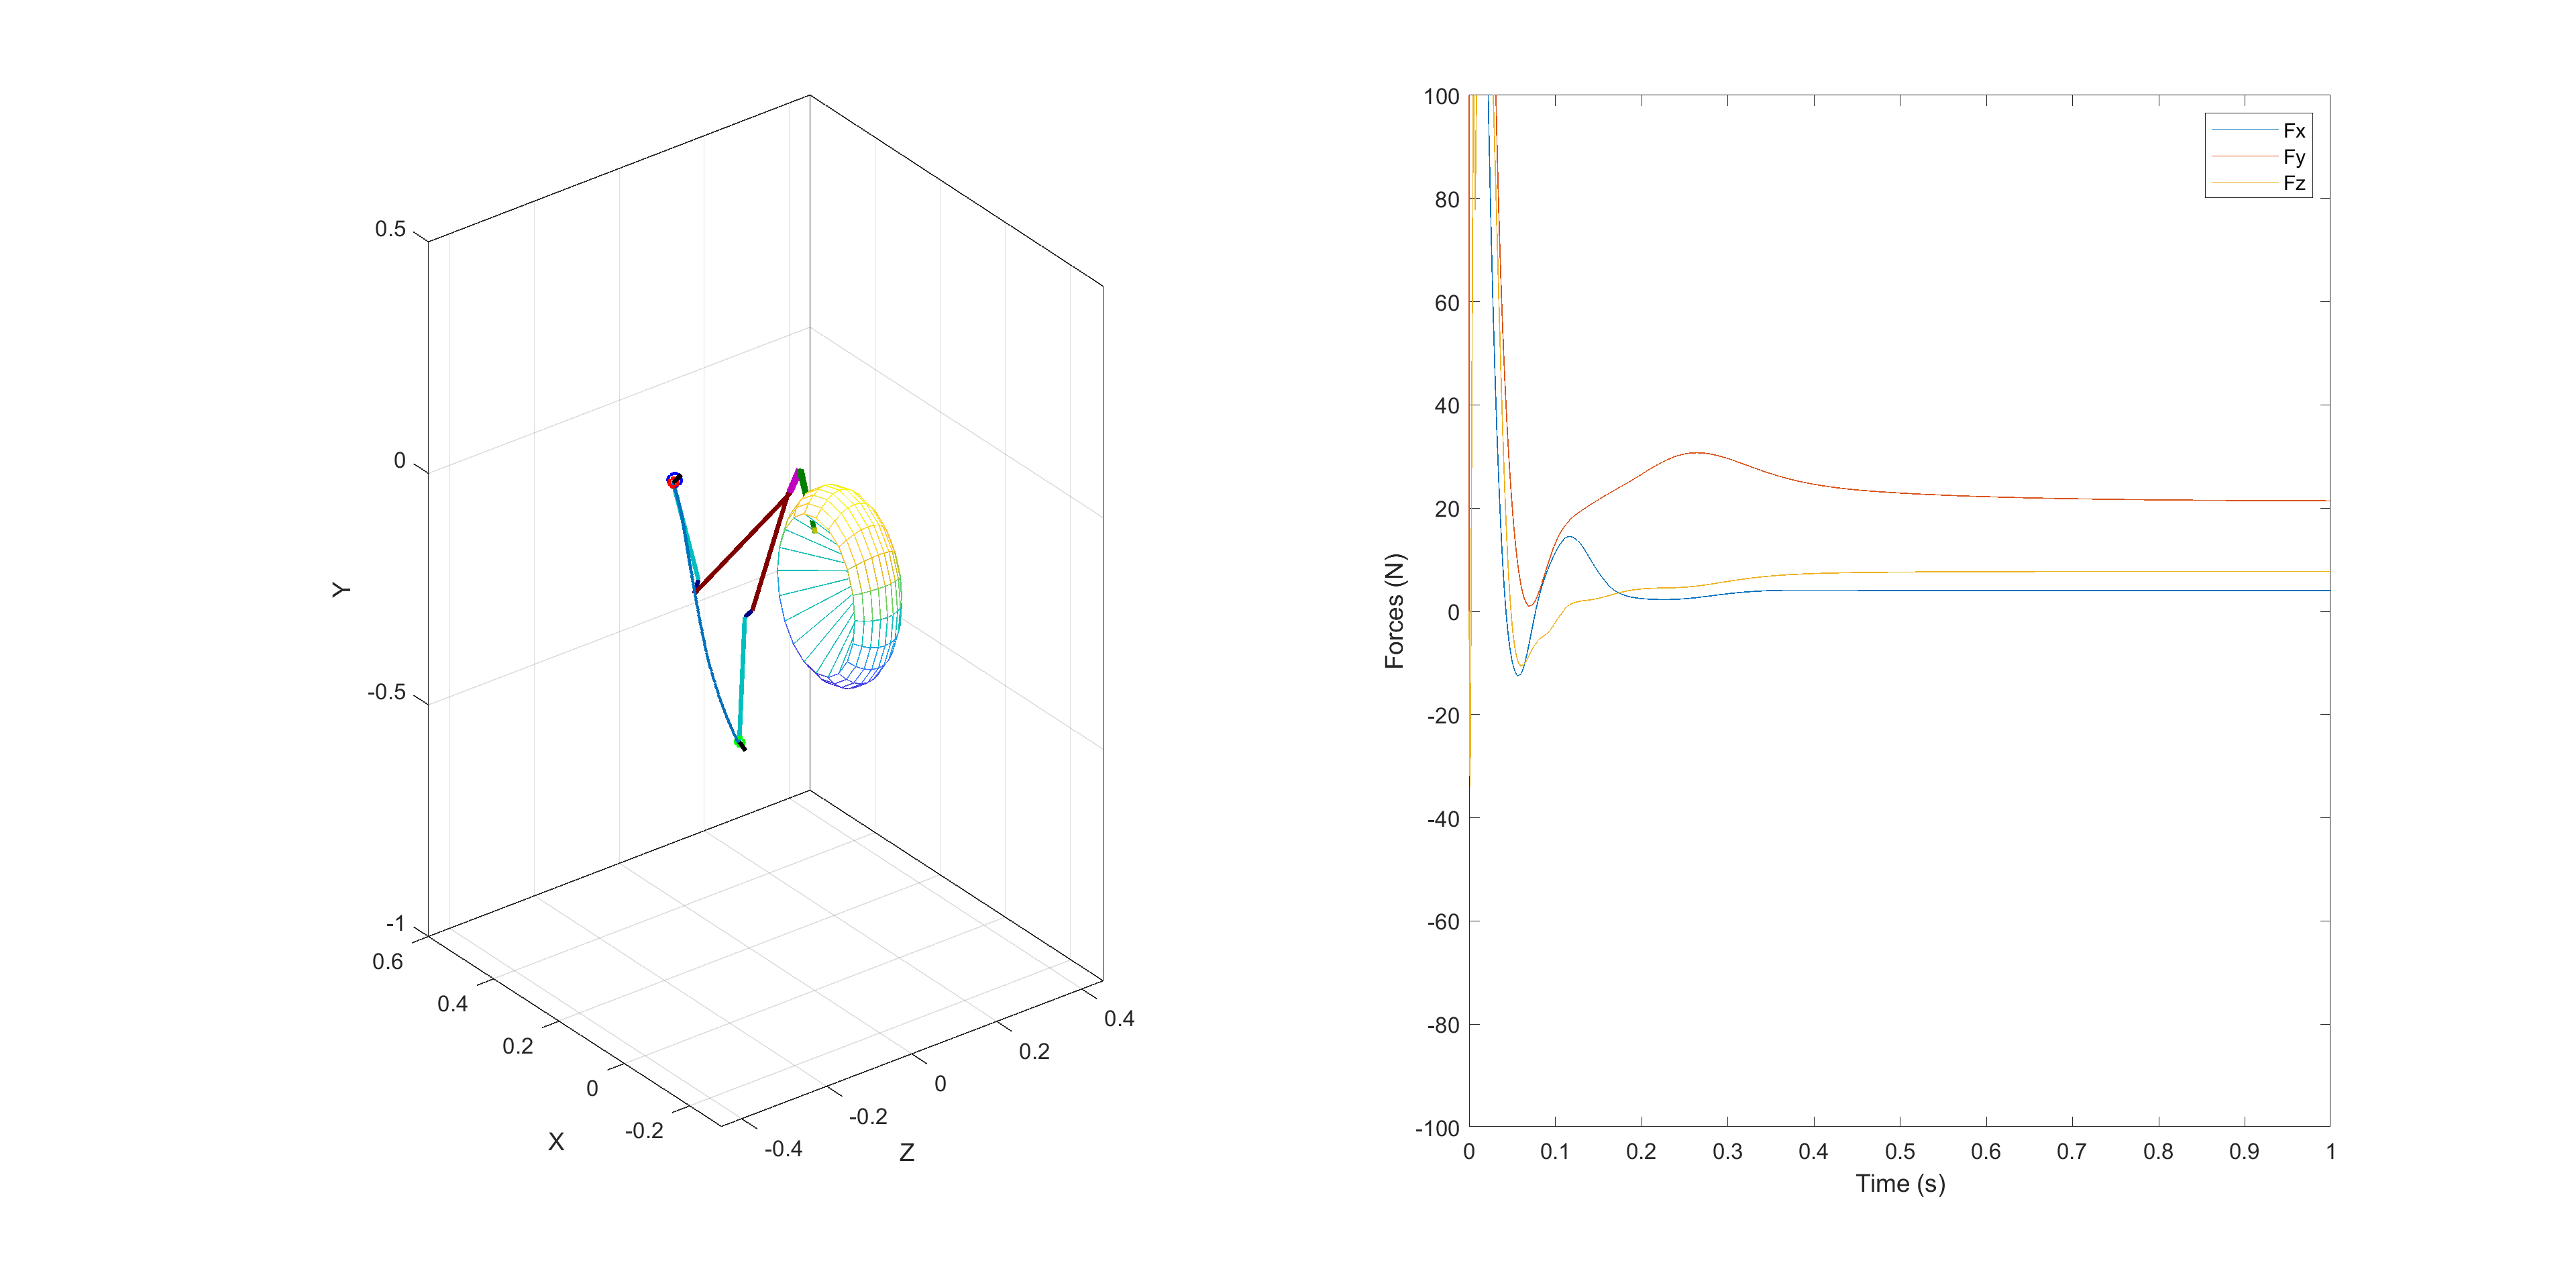
\includegraphics[width=0.7\linewidth]{Pictures/Results/1s_NoNeuralExcitation.png}
    \caption{PI Controller 1 second Simulation.}
\end{figure}


\newpage
\subsection{Support vs Non-Support}

Inspired on the work done in the research \cite{HSAC},\cite{QSC} and \cite{RTS} an arm support component was integrated into the PI controller to simulate the robotic arm that held the patient's arm as they suffered from spinal cord injury that did not allow them to lift their arm. In the scope a project, an arm support is added to mimic the common scenario observed in stroke survivors, where they leverage their own strength to support and stabilize their affected arm during rehabilitation exercises. The inclusion of this arm support component in the simulation is pivotal, as it offers a more realistic representation of the rehabilitation process. By accounting for the patient's inherent capability to self-support, the simulation ensures that the outcomes align closely with real-world scenarios, paving the way for more tailored and effective rehabilitation strategies. In the code of Matlab this arm support mechanism acts provides an additional force to guide the hand toward a desired position and maintaining stability by mitigating rapid or undesirable movements. 

As seen in the Figures below the arm support reduces oscillation improving the stability of the control. On the top image the figure shows the simulation to find the equivalent force without arm support and on the bottom figure the simulation with arm support. Figure \ref{fig:PINoExcitation} presents the case when no neural excitation is provided and Figure \ref{fig:PIExcitation} when Neural Excitation is given for one muscle.



\begin{figure}[h!] 
    \centering
    \begin{subfigure}[b]{0.7\linewidth}
       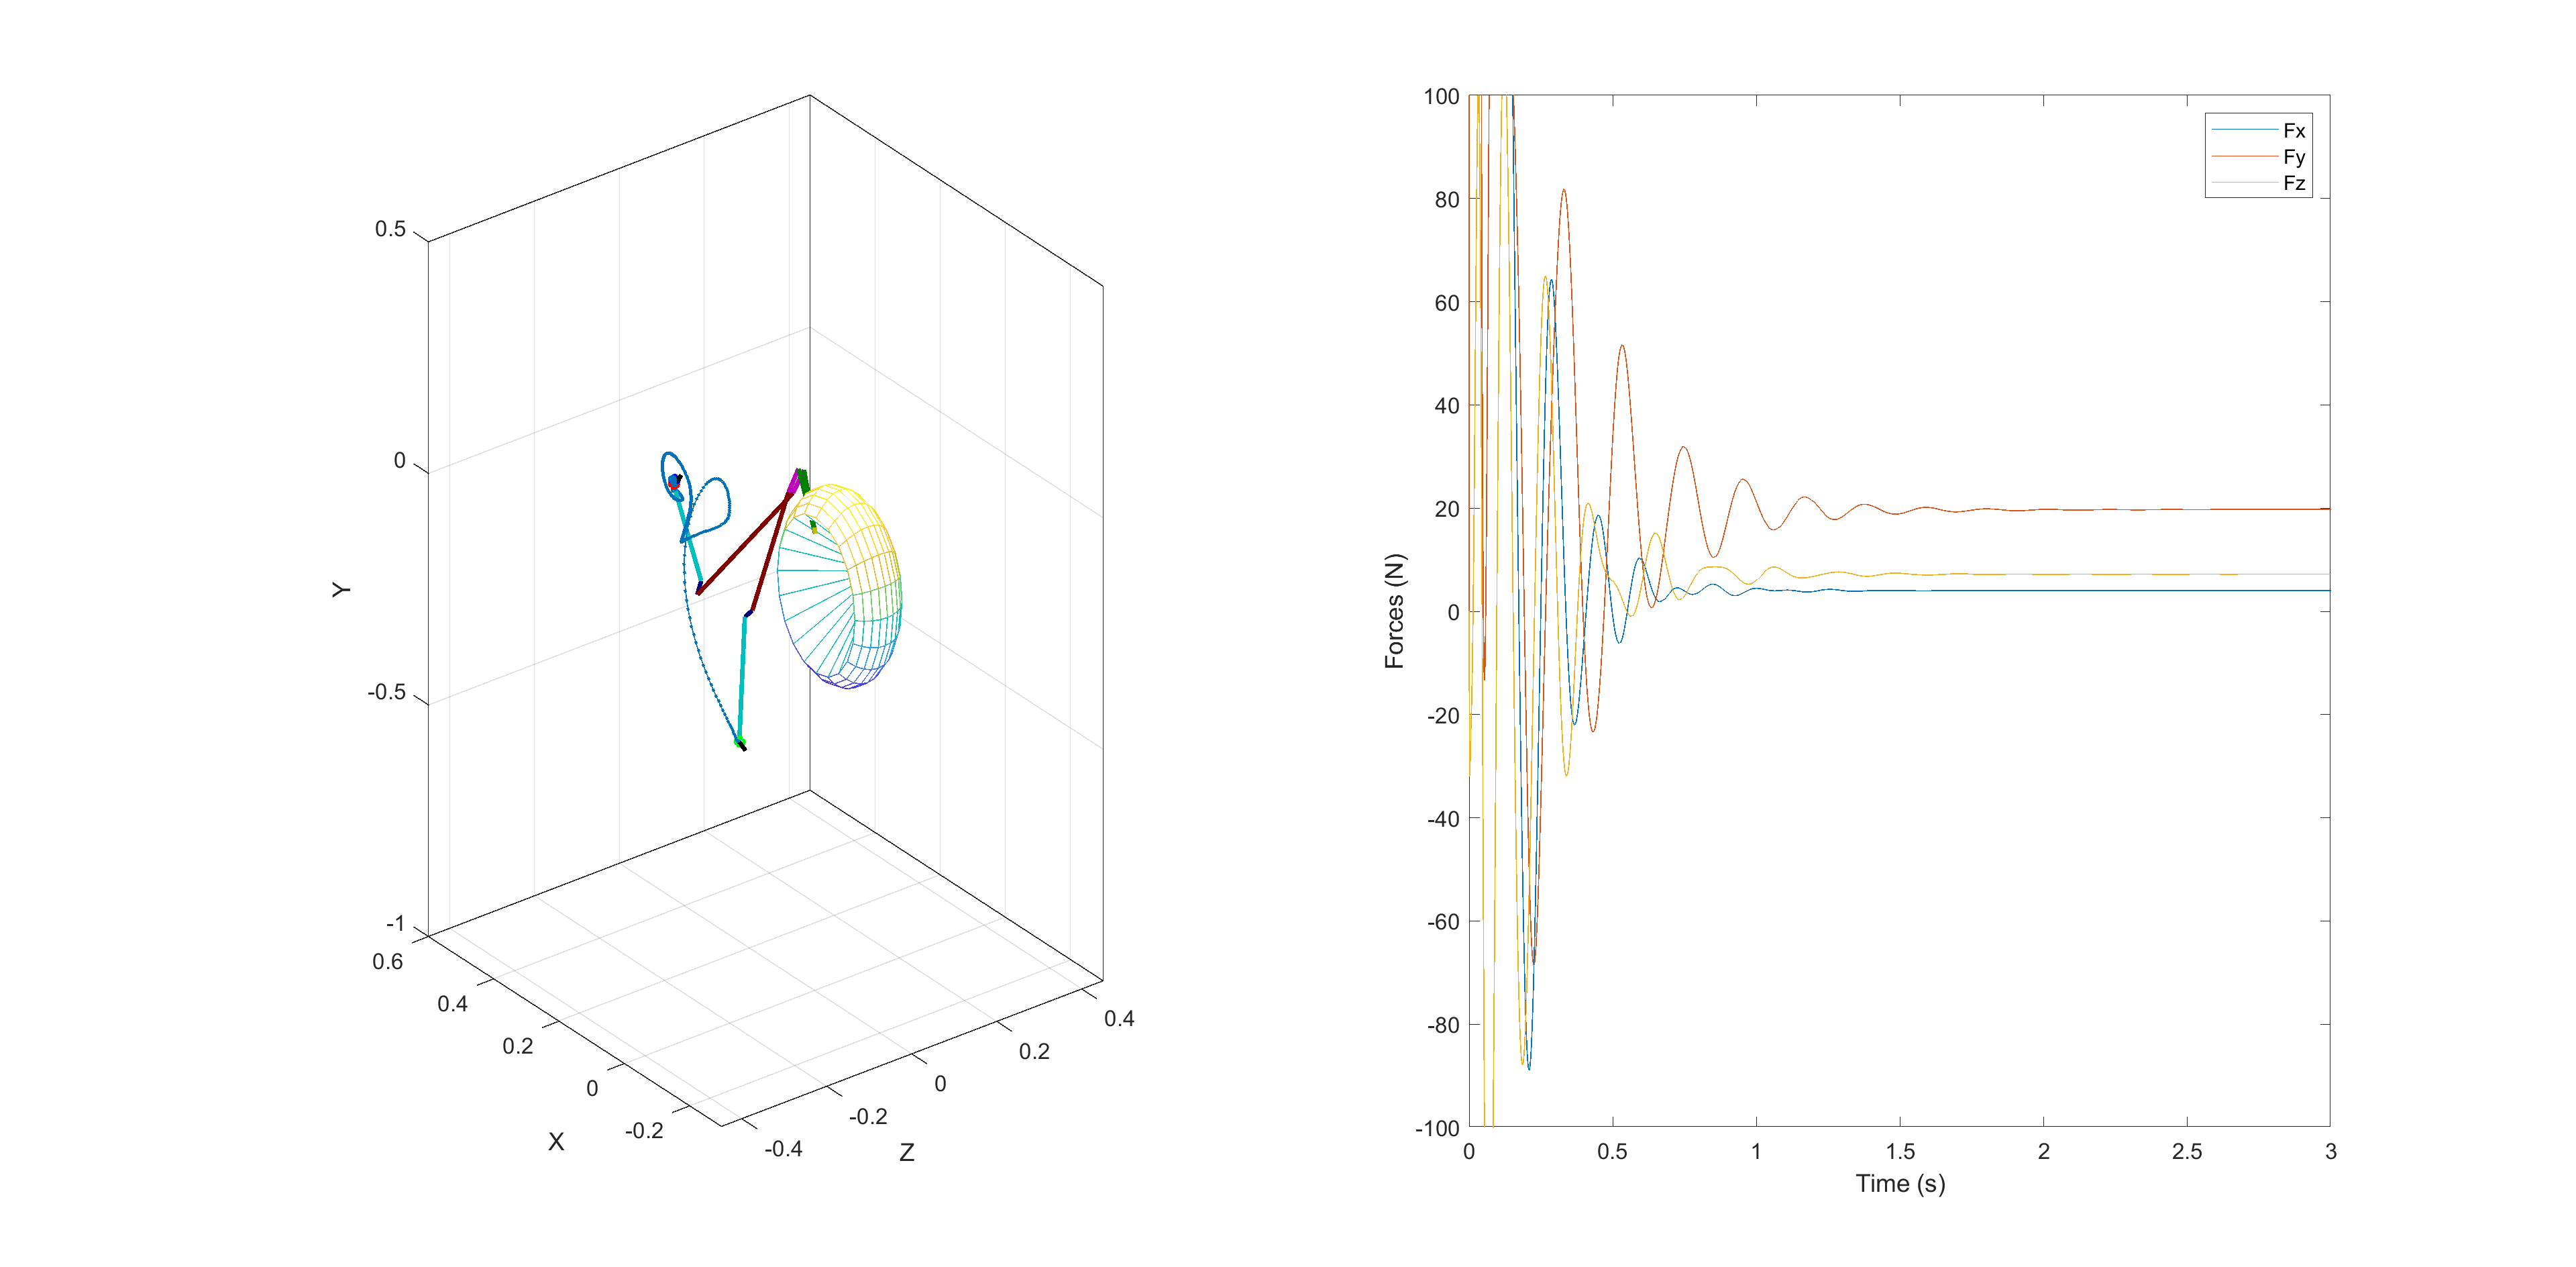
\includegraphics[width=\linewidth]{Pictures/Results/static_without_support.png}
        \caption{PI Controller Without Arm Support.}
    \end{subfigure}

    \vspace{1cm} % Adjust the space between the figures as needed
    \begin{subfigure}[b]{0.7\linewidth}            
        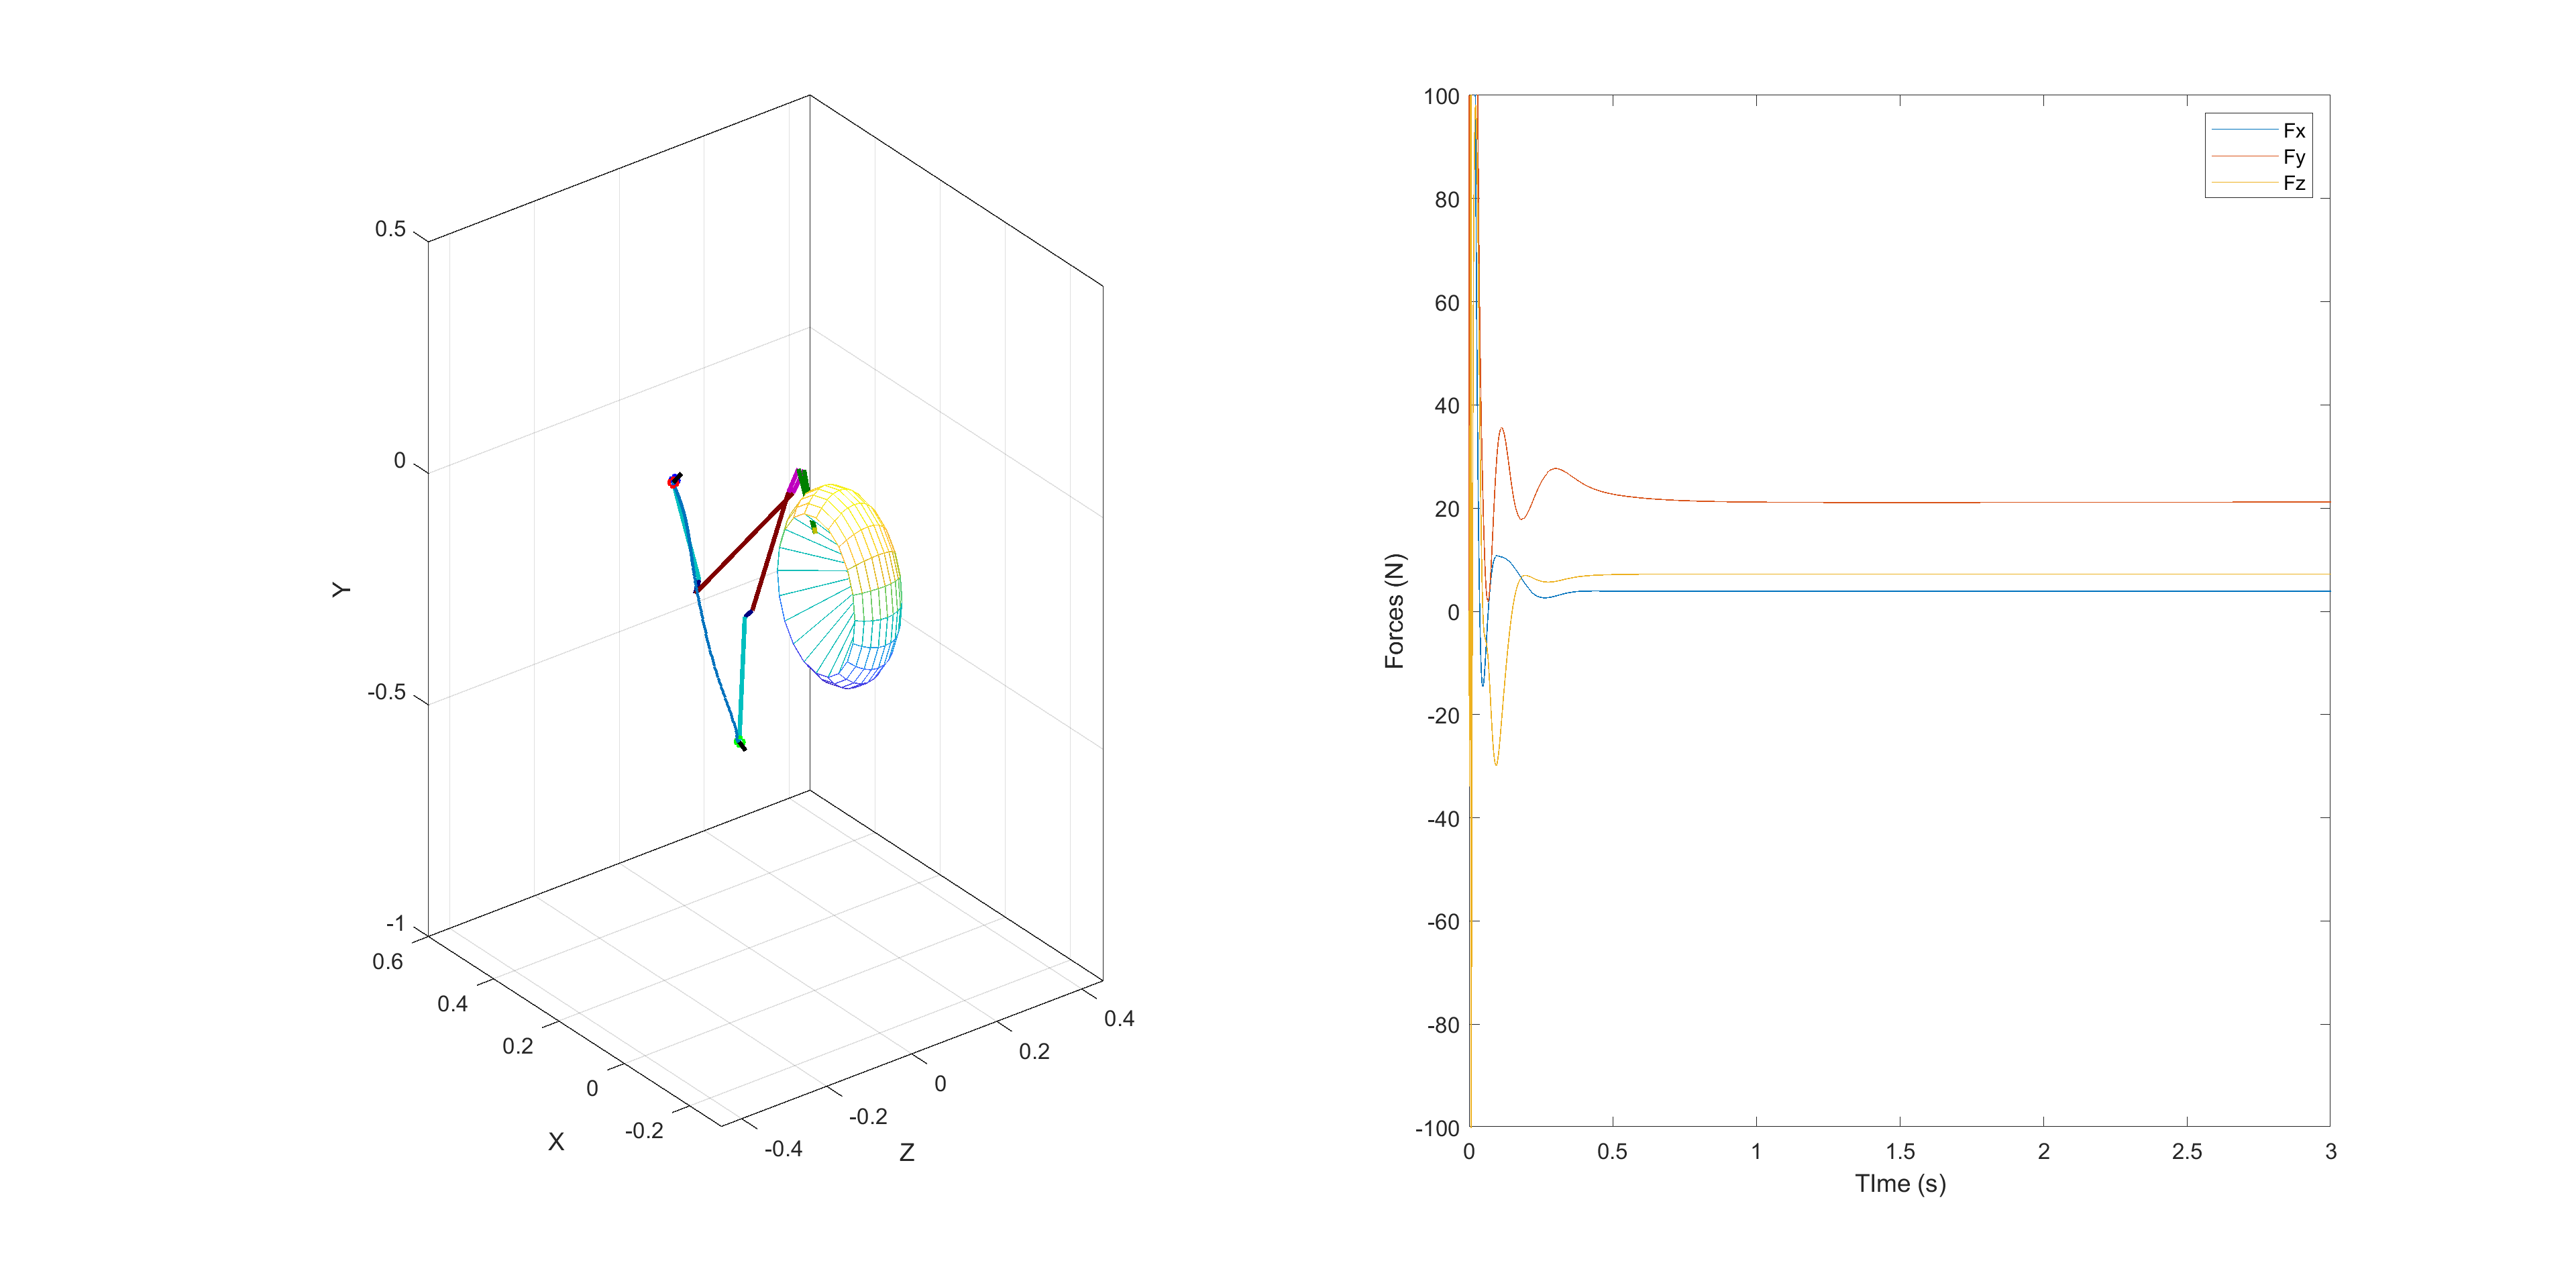
\includegraphics[width=\linewidth]{Pictures/Results/static_with_support.png}
        \caption{PI Controller With Arm Support.}
    \end{subfigure}

    \caption{PI Controller from Equilibrium Position to Static Position with No Muscles Excitation.}
    \label{fig:PINoExcitation}

\end{figure}


\begin{figure}[h!] 
    \centering
    \begin{subfigure}[b]{0.45\linewidth}
       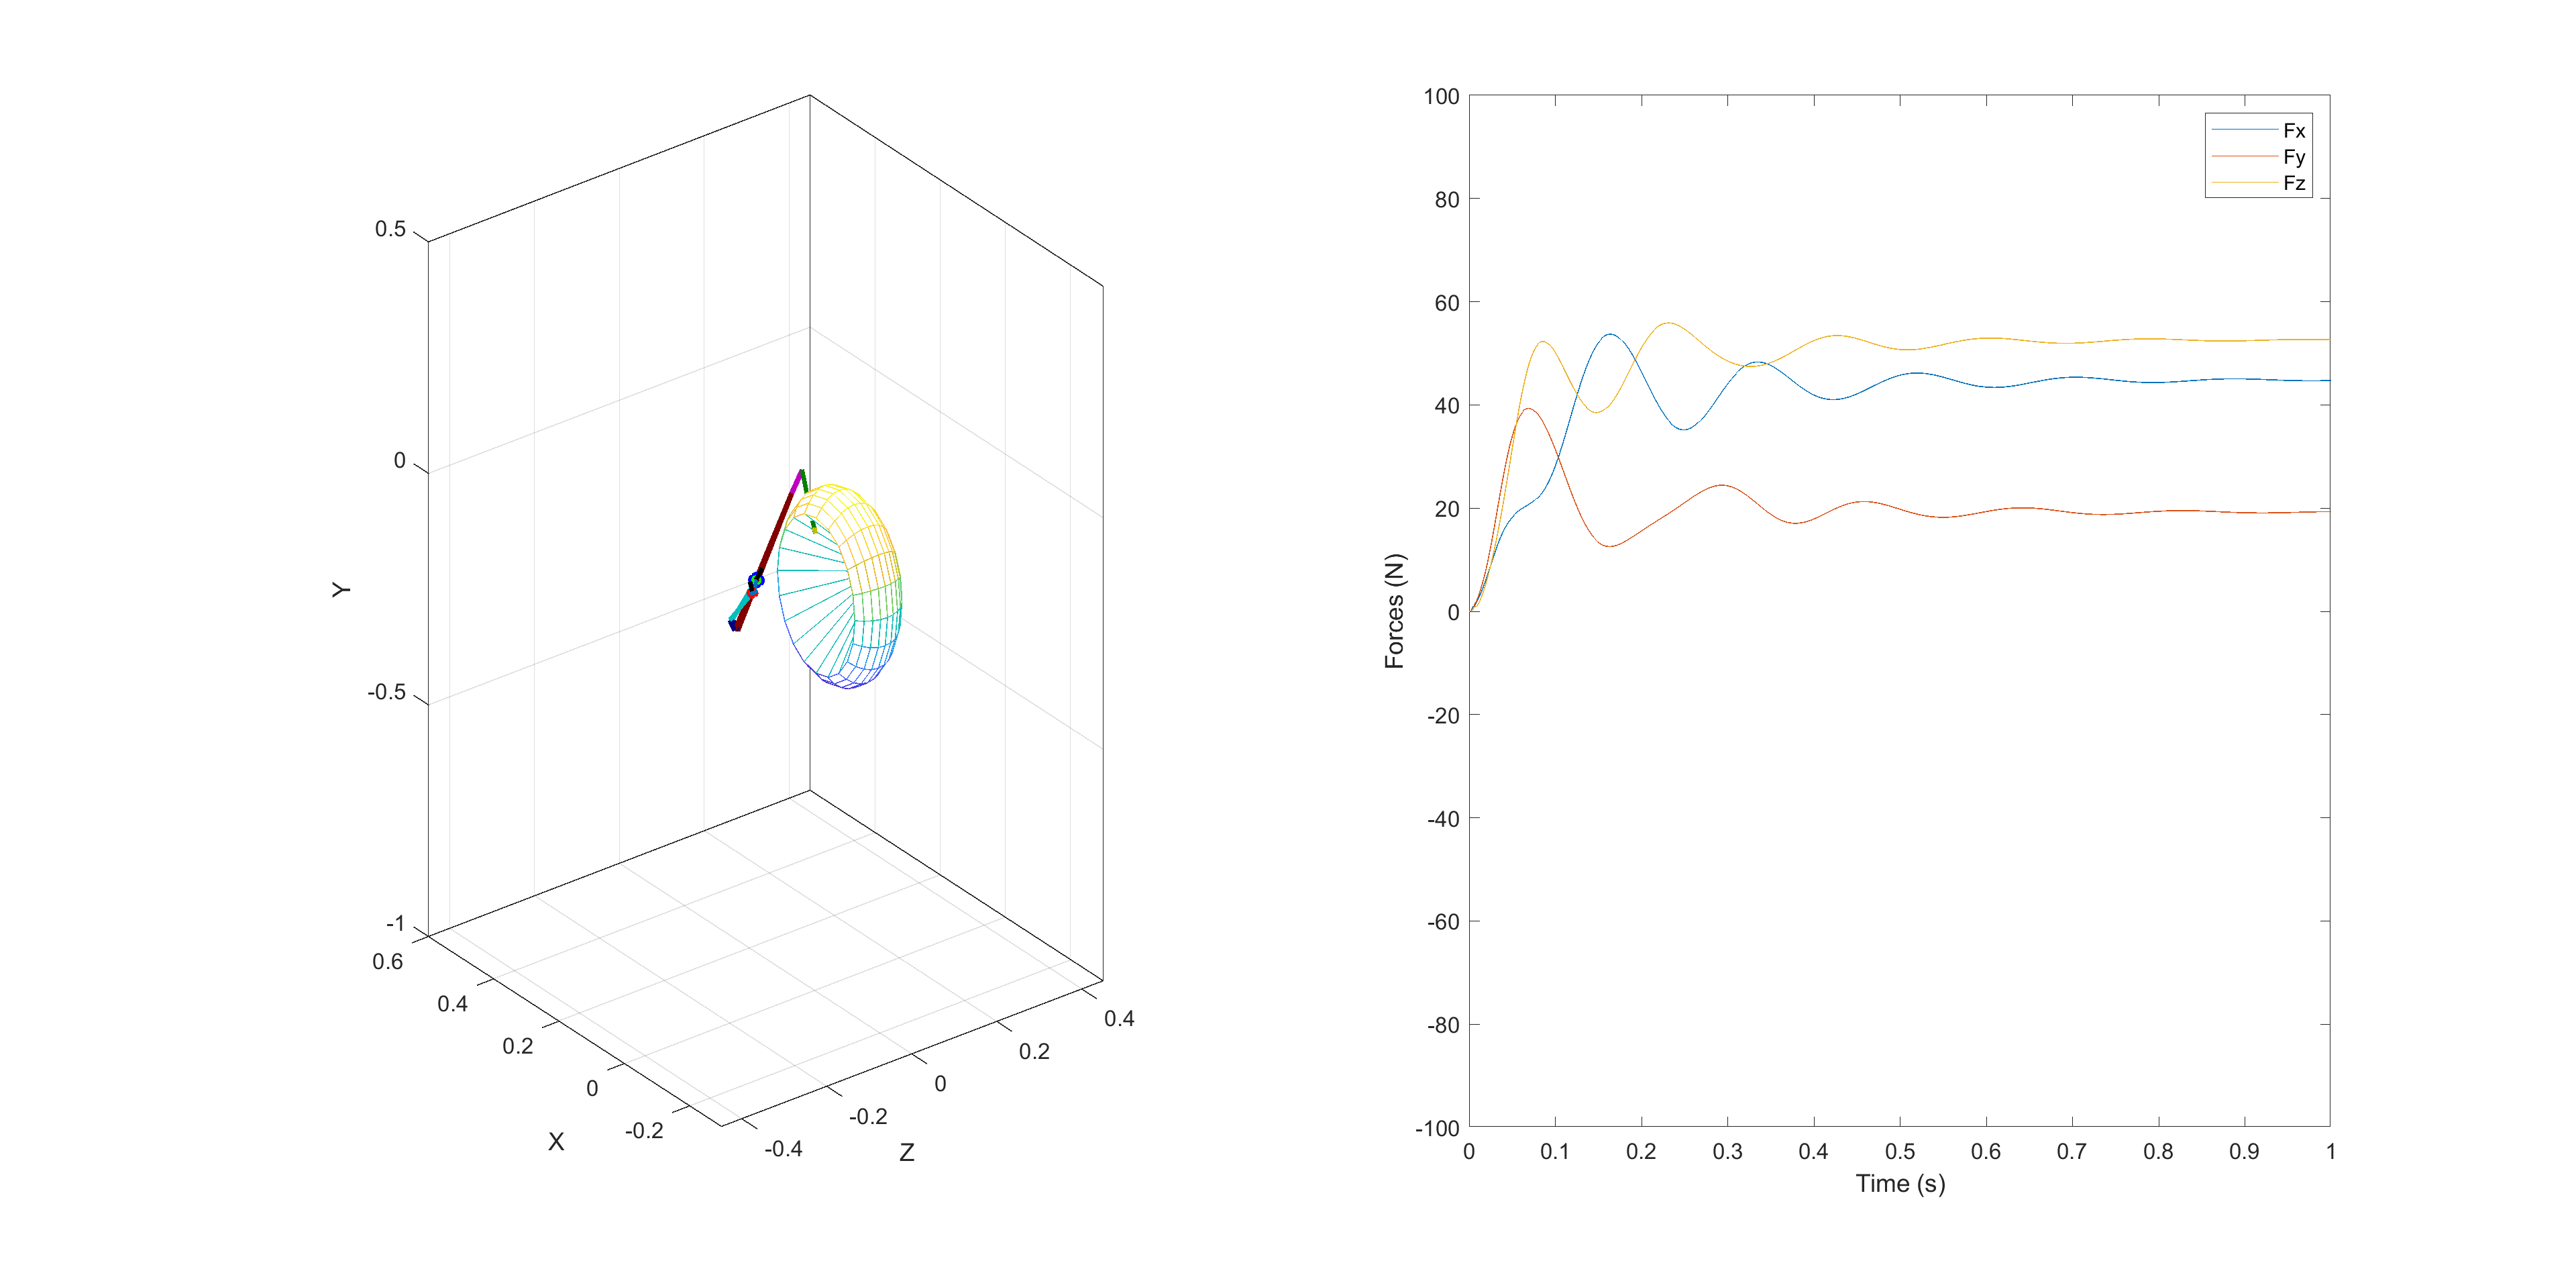
\includegraphics[width=1.1\linewidth]{Pictures/Results/stimuated_1_without_support.png}
        \caption{PI Controller Without Arm Support.}
    \end{subfigure}
    \hfill
    %\vspace{1cm} % Adjust the space between the figures as needed
    \begin{subfigure}[b]{0.45\linewidth}            
        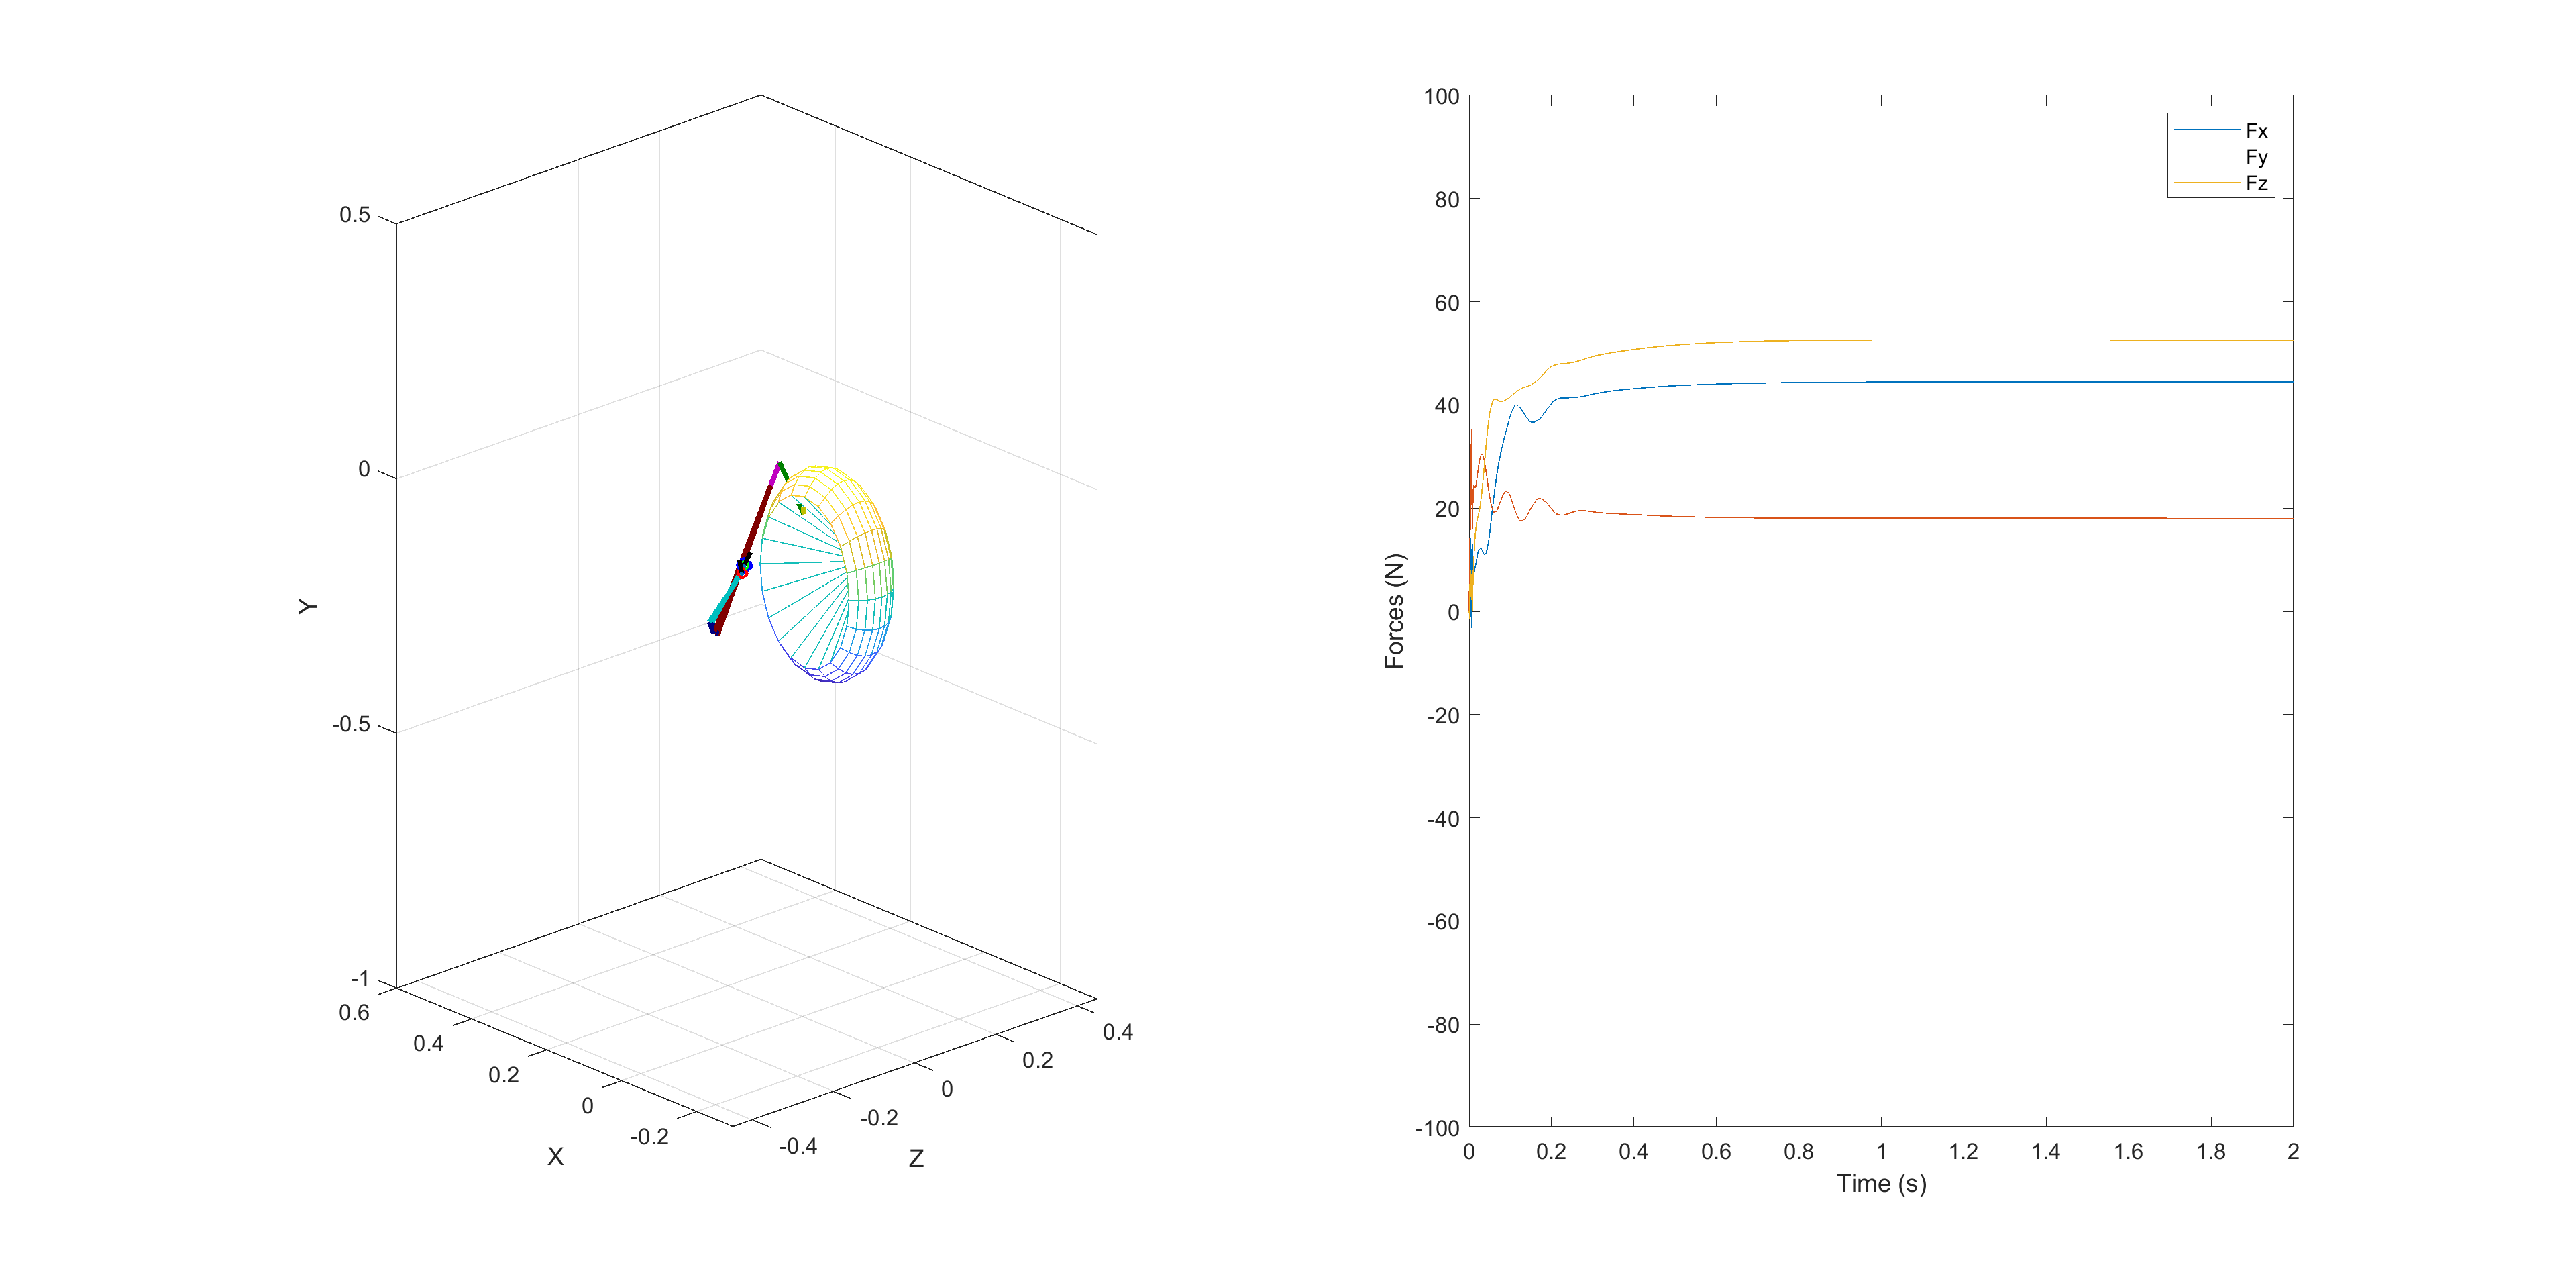
\includegraphics[width=1.1\linewidth]{Pictures/Results/stimuated_1_with_support.png}
        \caption{PI Controller With Arm Support.}
    \end{subfigure}

    \caption{PI Controller for holding Static Position with One Muscle Excitation.}
    \label{fig:PIExcitation}

\end{figure}